\section{Experiences and Numerical Analysis}

\subsection{Analysis of the ascent step convergence}
\begin{figure}
    \begin{subfigure}{.5\textwidth}
        \centering
        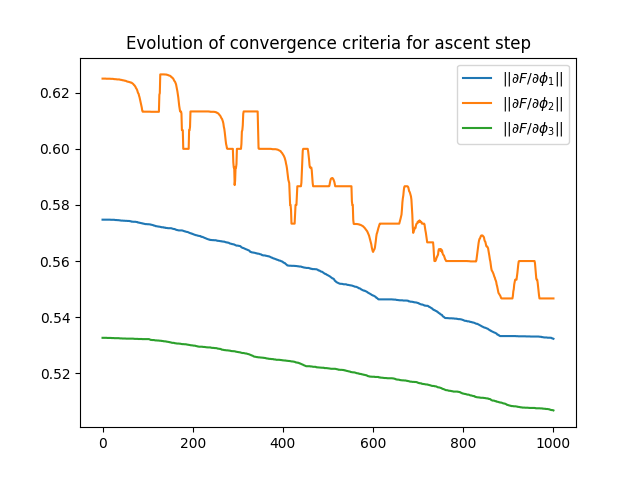
\includegraphics[width=\textwidth]{figures/ascent_criteria_n_samples16000.png}
    \end{subfigure}
    \begin{subfigure}{.5\textwidth}
        \centering
        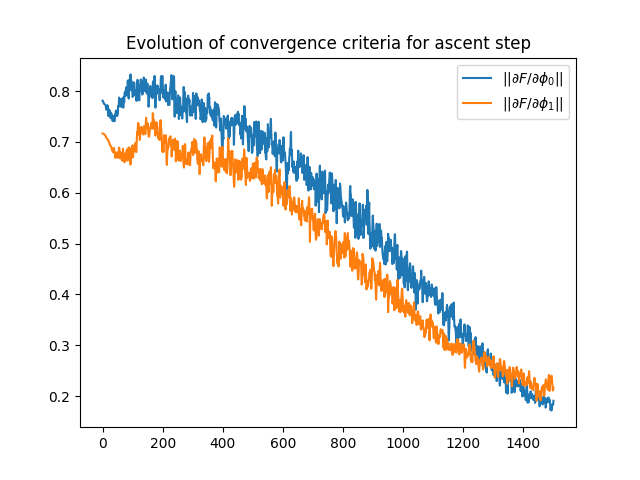
\includegraphics[width=\textwidth]{figures/ascent_criteria_msamples16000_iter0_1D_2skewnorm.png}
    \end{subfigure}
\end{figure}

\subsection{Numerical comparison}
\subsubsection{Computation of the barycenter with the optimal Monge map}
\label{sec:optimal_map}

\cite{peyre_computational_2020}
\subsubsection{Computation of the barycenter with Iterative Bregman Projections}
\begin{figure}
    \centering
    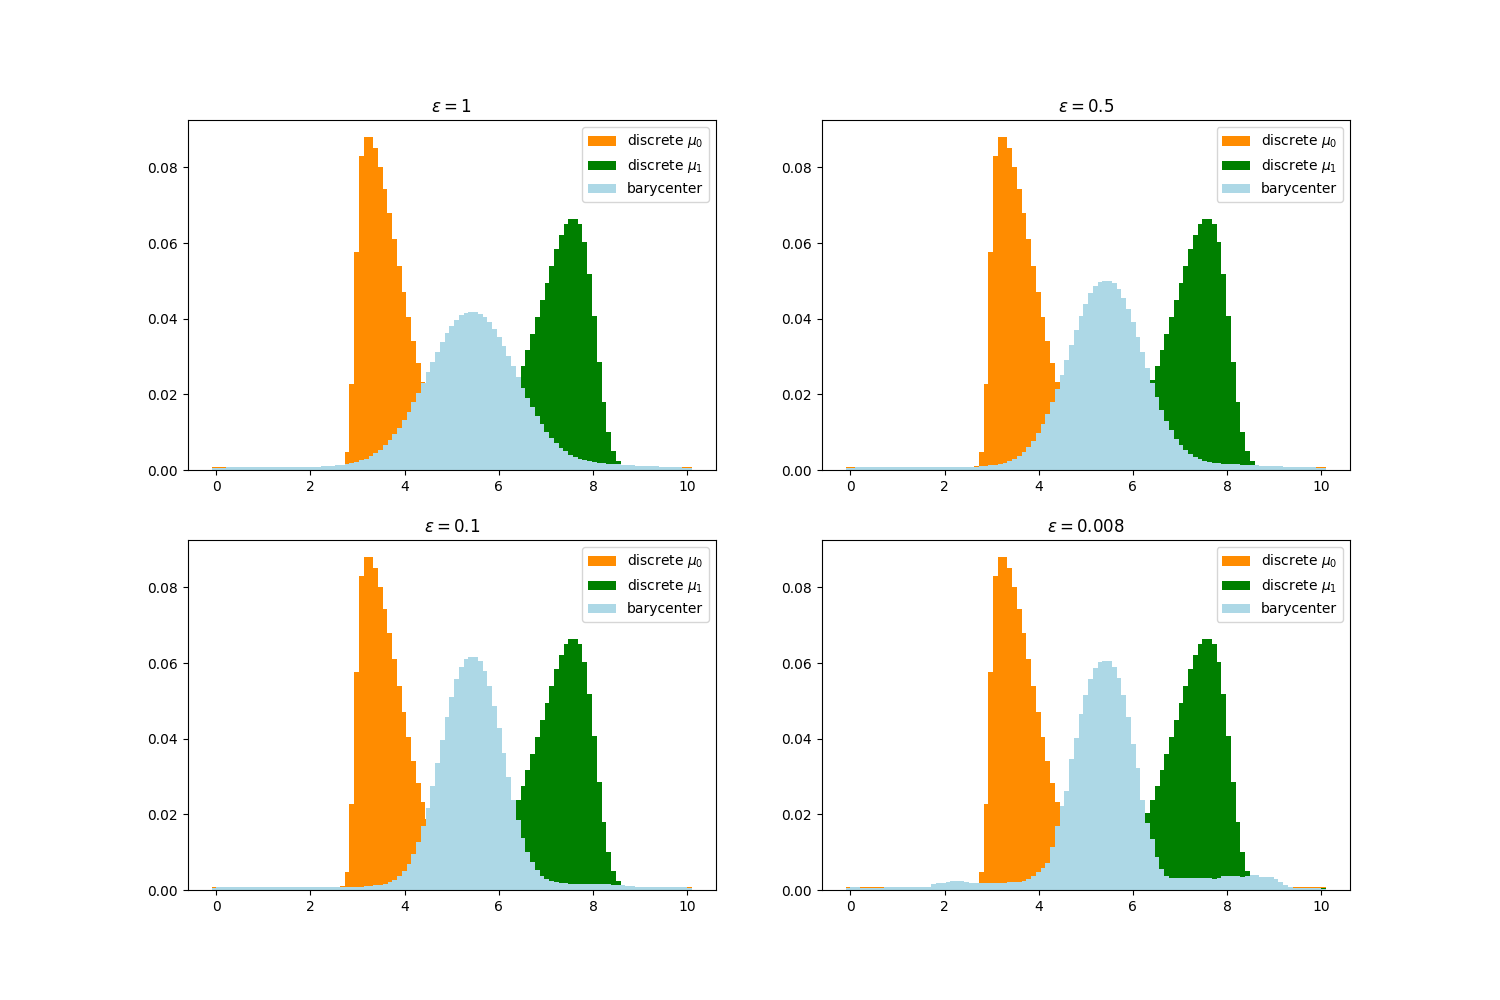
\includegraphics[width=\textwidth]{figures/sinkhorn_1D_2skew.png}
    \caption{Sinkhorn's interpolant}
    \label{fig:sinkhorn_1D_2skew}
\end{figure}

\subsubsection{Computation on free grid using POT toolbox}

\begin{figure}[!ht]
    \centering
    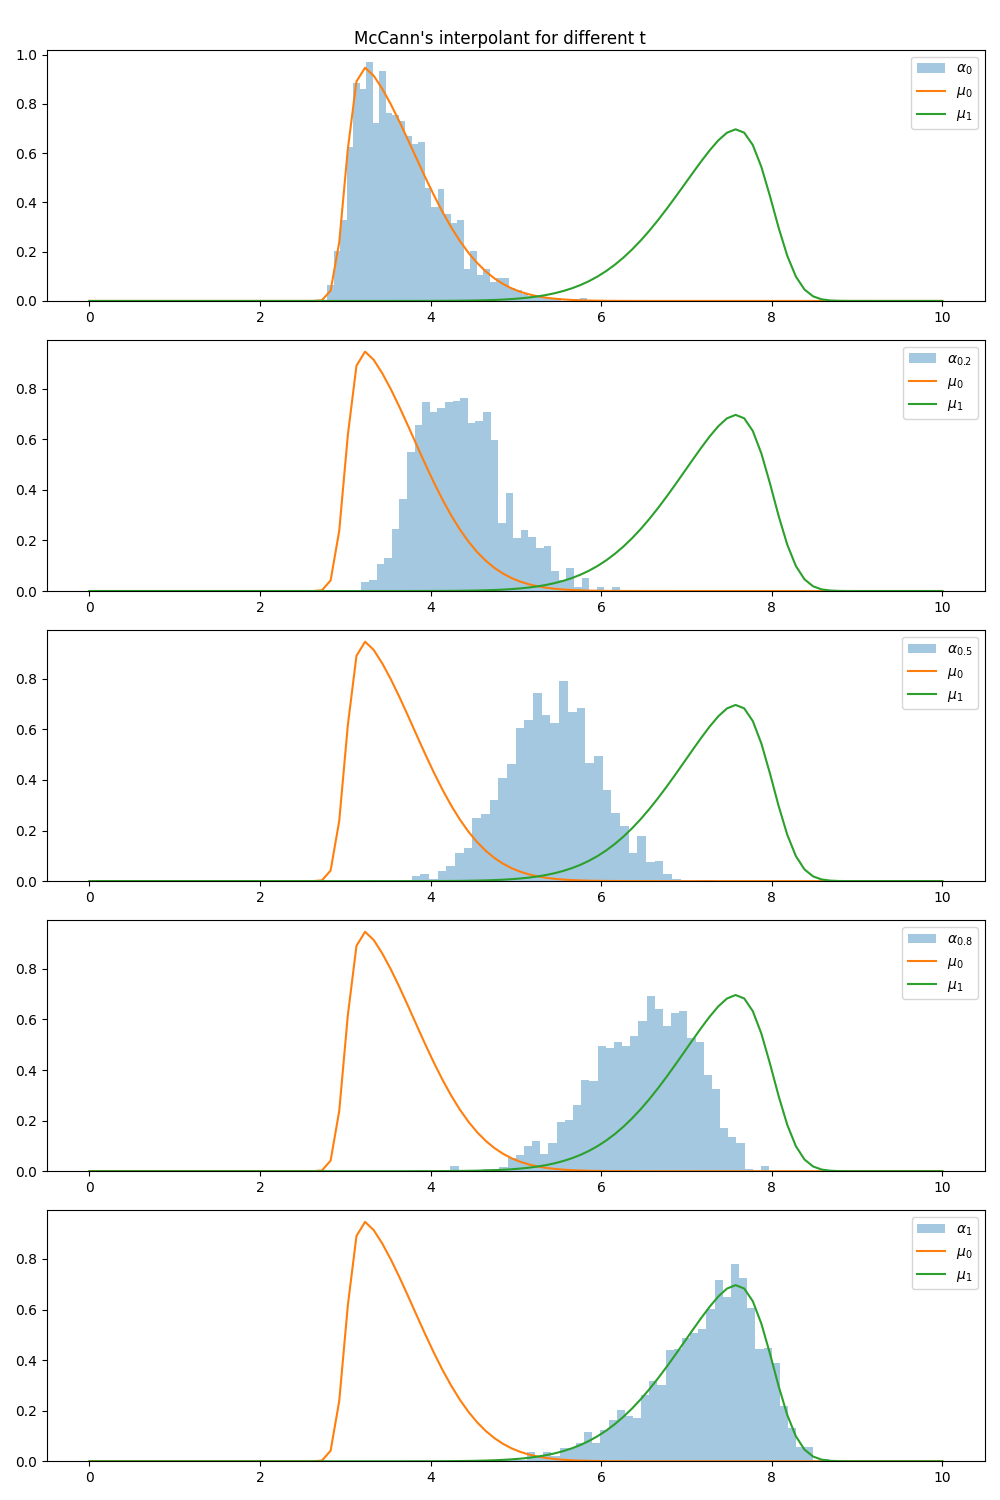
\includegraphics[width=\textwidth]{figures/mccann_1D_2skew.png}
    \caption{McCann's interpolant}
    \label{fig:mccann_1D_2skew}
\end{figure}
